\documentclass{article}

% if you need to pass options to natbib, use, e.g.:
%     \PassOptionsToPackage{numbers, compress}{natbib}
% before loading neurips_2024


% ready for submission
\PassOptionsToPackage{numbers, compress}{natbib}
\usepackage[preprint]{neurips_2024}
\makeatletter
\renewcommand{\@noticestring}{Preprint.}
\makeatother


% to compile a preprint version, e.g., for submission to arXiv, add add the
% [preprint] option:
%     \usepackage[preprint]{neurips_2024}


% to compile a camera-ready version, add the [final] option, e.g.:
%     \usepackage[final]{neurips_2024}


% to avoid loading the natbib package, add option nonatbib:
%    \usepackage[nonatbib]{neurips_2024}


\usepackage[utf8]{inputenc} % allow utf-8 input
\usepackage[T1]{fontenc}    % use 8-bit T1 fonts
\usepackage{hyperref}       % hyperlinks
\usepackage{amsmath}        % math
\usepackage{url}            % simple URL typesetting
\usepackage{booktabs}       % professional-quality tables
\usepackage{amsfonts}       % blackboard math symbols
\usepackage{nicefrac}       % compact symbols for 1/2, etc.
\usepackage{microtype}      % microtypography
\usepackage{xcolor}         % colors
\usepackage{graphicx}     % figure inclusion
\usepackage{float}
\usepackage{tikz}
\usetikzlibrary{positioning, arrows.meta, shapes, fit, calc}



\title{EgoBlind-RA: Towards Safer Egocentric Assistive AI for Blind Users via Risk-Adaptive Routing}

% The \author macro works with any number of authors. There are two commands
% used to separate the names and addresses of multiple authors: \And and \AND.
%
% Using \And between authors leaves it to LaTeX to determine where to break the
% lines. Using \AND forces a line break at that point. So, if LaTeX puts 3 of 4
% authors names on the first line, and the last on the second line, try using
% \AND instead of \And before the third author name.

\author{
  Julia Kim\thanks{Equal contribution.} \\
  Massachusetts Institute of Technology \\
  \texttt{julia225@mit.edu}
  \And
  Xander Backus\footnotemark[1] \\
  Massachusetts Institute of Technology \\
  \texttt{xabackus@mit.edu}
}

\begin{document}


\maketitle
\begin{abstract}
Blind and low-vision (BLV) users depend on visual assistance systems to navigate an unpredictable physical world, yet existing multimodal systems apply a uniform inference policy irrespective of query urgency. We present \textbf{EgoBlind-RA}, a risk-adaptive framework that classifies egocentric query-video pairs as \textit{urgent} or \textit{non-urgent} via a lightweight CLIP-based classifier and routes each query to a response calibrated to its safety stakes. Our classifier achieves 0.905 ROC-AUC on the held-out test set. We compare two LoRA-fine-tuned architectures of Kimi-VL-A3B-Instruct on the EgoBlind benchmark: a bifurcated design with separate urgent and non-urgent adapters, and a unified prompt-tag-conditioned design. Urgency-conditioned SFT against carefully selected reference targets substantially improves over a uniform-policy baseline in both. Surprisingly, DPO regresses SFT in the unified setting whilst proving productive in the bifurcated setting, where the best result mixes an SFT urgent adapter with a DPO non-urgent adapter. The unified adapter is also robust to noisy CLIP routing at deployment, matching oracle composite loss despite 21.5\% test-time tag flips. Together, these results suggest the value of preference-pair-based alignment and the cost of classifier noise both depend sharply on architectural regime.
\end{abstract}

\section{Introduction} Vision-language models (VLMs) have advanced rapidly, yet their development has largely centered on users with full sensory access. For the $\sim$253M people worldwide living with visual impairment \cite{bourne2017magnitude}, AI systems that interpret egocentric video and answer natural-language questions about the immediate environment offer a transformative opportunity to support independence and personal safety. Benchmarks for this setting --- EgoBlind \cite{xiao2025egoblind} and VizWiz \cite{bigham2010vizwiz} --- have begun to expose challenges specific to blind and low-vision (BLV) users: off-centre regions of interest, ambiguous spatial context, motion blur, and information needs ranging from casual to life-critical. Performance here matters beyond academic interest because the cost of a misleading answer is asymmetric, and in the safety-critical case, severe.

Yet state-of-the-art multimodal systems apply a uniform inference policy to every query, regardless of stakes. Consider two questions a blind user might ask: \textit{``Is there a step in front of me?''} signals an immediate physical hazard and demands a fast, conservative response; \textit{``What brand of cereal is this?''} tolerates a slower, more deliberative one. Models such as LLaVA \cite{liu2023llava} and InstructBLIP \cite{dai2023instructblip} treat the two identically, and the cost runs in both directions: excessive caution degrades usability on routine queries, whilst insufficient urgency on safety-critical ones risks physical harm. Urgency, moreover, is not determined by text alone --- \textit{``Is there anything in my way?''} carries very different stakes at the edge of a subway platform than in one's kitchen --- so any effective response policy must condition jointly on the question and the visual scene. To our knowledge, no prior assistive system jointly classifies visual urgency and routes queries to risk-stratified response policies.

In this paper, we propose \textbf{EgoBlind-RA}, a risk-adaptive egocentric visual assistance framework for BLV users. EgoBlind-RA is a two-stage pipeline: a lightweight CLIP-based classifier predicts whether each query--video pair is \textit{urgent} or \textit{non-urgent}, and the predicted urgency conditions a fine-tuned VLM. We investigate two architectures: a bifurcated design with separate urgent and non-urgent Low-Rank Adaptation (LoRA) adapters (\textbf{Approach 1}), and a unified single-adapter design conditioned by an urgency prompt-tag (\textbf{Approach 2}). Both are optimized under a regime-specific composite loss balancing accuracy, assistive utility, and generation latency.

We make three contributions. First, a frozen-backbone CLIP classifier predicts query urgency from joint video--text representations, reaching 0.905 ROC-AUC on the test set. Second, urgency-conditioned SFT with length-asymmetric reference targets --- shortest-correct for urgent queries, longest-correct for non-urgent --- substantially outperforms the uniform-policy baseline in both architectures. Third, two central design choices depend sharply on adapter architecture: DPO regresses SFT in the unified design but is productive in the bifurcated one, and the unified design absorbs CLIP routing errors at deployment (matching oracle composite loss despite 21.5\% tag flips) whereas the bifurcated design does not. These results suggest that alignment method, classifier robustness, and adapter architecture must be co-designed.

\section{Related Work} \label{sec:related} 
\paragraph{Visual assistance for BLV users.}
VizWiz \cite{bigham2010vizwiz} introduced an early assistive VQA system in which BLV users photographed their surroundings and asked questions that were answered by crowd workers. This work highlighted challenges characteristic of BLV-generated images, including poor framing, motion blur, and queries spanning both low- and high-stakes situations. The setting was later formalized as a large-scale VQA benchmark \cite{gurari2018vizwiz} that demonstrated BLV-generated images are substantially more difficult for existing models than standard VQA inputs. More recently, EgoBlind \cite{xiao2025egoblind} extended the problem to egocentric video; we adopt EgoBlind as our evaluation dataset. However, none of these benchmarks evaluates whether models adapt their behavior to the urgency or safety-criticality of user queries.

\paragraph{Egocentric video understanding.}
Ego4D \cite{grauman2021ego4d} introduced a large corpus of egocentric video supporting tasks such as episodic memory, action anticipation, and future forecasting. Embodied Question Answering \cite{das2018embodied} introduced a setting in which an agent must navigate through an environment to obtain the information needed to answer a query. However, both settings assume sighted users and treat all queries uniformly, without accounting for differences in urgency or safety criticality.

\paragraph{VLMs and efficient adaptation.}
Recent VLMs, including LLaVA \cite{liu2023llava}, InstructBLIP \cite{dai2023instructblip}, Qwen-VL \cite{bai2023qwenvl}, and Kimi-VL \cite{kimivl2025}, achieve strong out-of-the-box performance on visual question answering tasks. We employ Kimi-VL as our base model. Our urgency classifier is built on representations from CLIP \cite{radford2021clip}, whilst LoRA \cite{hu2022lora} enables efficient fine-tuning of multi-billion-parameter models on a single GPU.

\paragraph{Alignment and preference optimization.}
Reinforcement Learning from Human Feedback (RLHF) \cite{ouyang2022instructgpt} aligns language models to human preferences using a reward model trained on pairwise comparisons. DPO \cite{rafailov2023dpo} simplifies this process by optimizing directly from preference pairs, and is now widely adopted. Variants include Kahneman--Tversky Optimization (KTO) \cite{ethayarajh2024kto}, which uses scalar utility labels instead of pairwise comparisons; Reinforcement Learning from AI Feedback (RLAIF) \cite{lee2023rlaif}, which replaces human labels with AI feedback; and Group Relative Policy Optimization (GRPO) \cite{shao2024deepseekmath}, which scores groups of sampled responses against a learned baseline rather than pairwise. We apply DPO with urgency-conditioned preference pairs and find that its effect depends sharply on adapter architecture --- a failure mode not previously reported for short, vision-grounded VQA.

\paragraph{Risk-aware inference.}
Several lines of work adapt model behavior to input risk: models can abstain when uncertain \cite{whitehead2022reliable}, estimate uncertainty using semantic entropy \cite{kuhn2023semantic}, or allocate more compute to difficult inputs \cite{schuster2022confident}. Importantly, these approaches are text-only and do not incorporate a learned visual urgency signal.

\paragraph{How our work differs.}
EgoBlind-RA is, to our knowledge, the first system to classify urgency from egocentric video and route queries to risk-stratified response policies in the assistive setting. We further show that DPO's effect on SFT, and the deployment cost of classifier errors, both depend sharply on adapter architecture, a contrast to prior alignment and BLV work that treats these decisions in isolation.


\section{Problem Statement} \label{sec:problem}
Let $\mathbf{x} = (v, q)$ denote a video-query pair, where $v \in \mathcal{V}$ is an egocentric video clip and $q \in \mathcal{Q}$ is a natural language query from a BLV user. Each pair has a binary urgency label $u \in \{0, 1\}$ and a reference answer set $\mathcal{Y}^{*} = \{y_1^*, \dots, y_K^*\}.$ EgoBlind-RA solves two coupled subproblems: 
\begin{enumerate}
    \item[(1)] learn an \textbf{urgency classifier} $f_\theta : \mathcal{V} \times \mathcal{Q} \rightarrow \{0,1\}$; 
    \item[(2)] learn a \textbf{conditional response generator} $g_\phi : \mathcal{V} 
\times \mathcal{Q} \times \{0,1\} \rightarrow \mathcal{A}$, whose objective depends on the predicted urgency $\hat{u} = f_\theta(\mathbf{x})$. We instantiate $g$ in two ways: Approach 1 trains separate generators $g_{\phi_u}, g_{\phi_{n}},$ and selects between them by $\hat{u}$; Approach 2 trains a single generator $g_{\phi}$ that takes $\hat{u}$ as an input prompt-tag. 
\end{enumerate}
The objective for $g$ is regime-specific: a composite loss balancing accuracy, assistive utility, and generation latency for urgent queries, and an accuracy-and-utility-only loss for non-urgent ones. We define these objectives in Section~\ref{sec:composite_loss}. 

\section{Proposed Method}\label{sec:approach}
As illustrated in Figure~\ref{fig:pipeline}, EgoBlind-RA operates as a two-stage pipeline: (i) an urgency classifier predicts the risk level of each query, and (ii) a conditional response generator produces an answer matched to the predicted urgency regime. We investigate two instantiations of the second stage, motivated by an open architectural question: should risk-adaptive behaviour be encoded \emph{structurally}, via separate adapters, or \emph{procedurally}, via a single adapter conditioned on a prompt tag? The two approaches differ only at this point in the pipeline; classifier, loss, base model, and inference-time routing signal are otherwise shared.

\begin{figure}[H]
\centering
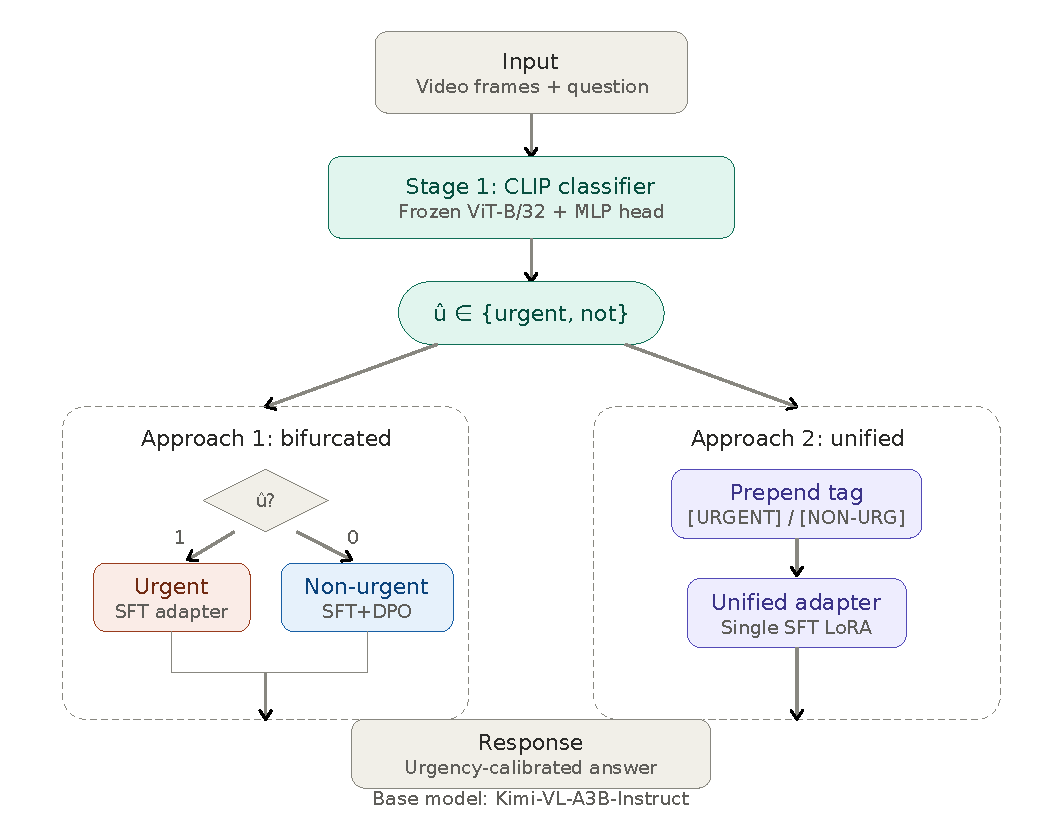
\includegraphics[width=0.75\columnwidth]{pipeline.pdf}
\caption{EgoBlind-RA pipeline. A CLIP-based classifier predicts query urgency from the joint video--text representation; the predicted urgency then routes to one of two architectural variants. Approach~1 selects between separate urgent and non-urgent LoRA adapters. Approach~2 prepends an urgency tag to a single unified adapter. Both are scored under the same regime-specific composite loss.}
\label{fig:pipeline}
\end{figure}

\subsection{Stage 1: Urgency Classification}
Given a video--query pair $\mathbf{x} = (v, q)$, we train a lightweight classifier $f_\theta$ to predict the binary urgency label $\hat{u} \in \{0,1\}$. The model uses a frozen CLIP ViT-B/32 backbone: $K$ frames sampled around the query timestamp are encoded individually, mean-pooled to produce a single visual embedding, and concatenated with the CLIP text embedding of the question. The fused representation is passed to a two-layer MLP head trained with binary cross-entropy.

Keeping the classifier lightweight lets it act as a fast preprocessing step before the response generator; freezing the backbone preserves CLIP's pretrained multimodal representations without end-to-end fine-tuning. We use a default decision threshold of 0.5 at inference; threshold tuning to reduce false negatives is discussed as future work (Section~\ref{sec:conclusion}). Architectural and training details appear in Section~\ref{sec:experiments}, with results in Section~\ref{sec:clip_results}.

\subsection{Stage 2: Urgency-Conditioned Response Generation}
We compare two architectural instantiations of the response generator (Figure~\ref{fig:pipeline}), differing only in how urgency is incorporated. Both use the composite loss defined in Section~\ref{sec:composite_loss}.

\paragraph{\textit{Approach 1: Bifurcated adapters.}}
We train two separate LoRA adapters on a shared base model $\mathcal{M}$. The \textit{urgent adapter} $\phi_u$ is fine-tuned on $\mathcal{D}_u = \{(\mathbf{x}_i, y_i) : u_i = 1\}$ under the full loss $\mathcal{L}_{\text{urgent}}$, with the \emph{shortest} correct reference answer as target to encourage concise, actionable responses. The \textit{non-urgent adapter} $\phi_n$ is fine-tuned on $\mathcal{D}_n = \{(\mathbf{x}_i, y_i) : u_i = 0\}$ under $\mathcal{L}_{\text{acc}} + \mathcal{L}_{\text{util}}$ (no latency term), with the \emph{longest} reference answer as target. At inference, the classifier prediction $\hat{u}$ selects the adapter:
\begin{equation}
    y = \begin{cases}
        \mathcal{M}_{\phi_u}(\mathbf{x}) & \text{if } \hat{u} = 1, \\
        \mathcal{M}_{\phi_n}(\mathbf{x}) & \text{if } \hat{u} = 0.
    \end{cases}
\end{equation}
The hard-routing design lets each adapter specialize without compromising the other regime. It also makes the classifier a hard gate: a single misrouted query loads an adapter that has not seen its training distribution, with no graceful fallback. Section~\ref{sec:dpo_results} examines the deployment-time cost of this brittleness empirically.

\paragraph{\textit{Approach 2: Prompt-conditioned unified adapter.}}
A single LoRA adapter $\phi_{\text{uni}}$ is trained on the full dataset $\mathcal{D}_u \cup \mathcal{D}_n$, with urgency provided as a control tag prepended to the system prompt. The loss switches accordingly: $\mathcal{L}_{\text{urgent}}$ for \texttt{[URGENT]} examples and $\mathcal{L}_{\text{non-urgent}}$ for \texttt{[NON-URGENT]} examples (Section~\ref{sec:composite_loss}). This setup tests whether prompt conditioning alone is enough for a single model to learn risk-adaptive behaviour. Compared to Approach~1, it halves adapter storage and exposes both regimes to a single set of parameters during training, a design we expected to make the model more tolerant of routing noise but potentially less able to specialize on either regime. Whether this trade-off favours unified or bifurcated training is an empirical question we resolve in Sections~\ref{sec:sft_results}--\ref{sec:dpo_results}.

\subsection{Composite Loss}\label{sec:composite_loss}
The composite loss is regime-specific. For urgent queries ($\hat{u} = 1$),
\begin{equation}
    \mathcal{L}_{\text{urgent}} = \alpha\,\mathcal{L}_{\text{acc}} + \beta\,\mathcal{L}_{\text{util}} + \gamma\,\mathcal{L}_{\text{lat}}, \qquad \alpha + \beta + \gamma = 1, \quad \alpha, \beta, \gamma > 0.
\end{equation}
For non-urgent queries ($\hat{u} = 0$), the latency term is dropped and the remaining weights are renormalized:
\begin{equation}
    \mathcal{L}_{\text{non-urgent}} = \frac{\alpha}{\alpha + \beta}\,\mathcal{L}_{\text{acc}} + \frac{\beta}{\alpha + \beta}\,\mathcal{L}_{\text{util}}.
\end{equation}

\paragraph{Accuracy.} $\mathcal{L}_{\text{acc}}$ penalizes semantic mismatch between $y$ and the closest reference in $\mathcal{Y}^*$:
\begin{equation}
    \mathcal{L}_{\text{acc}}(y, \mathcal{Y}^*) = 1 - \max_{k \in [K]} S(y, y_k^*),
\end{equation}
where $S(\cdot,\cdot) \in [0,1]$ is token-overlap F1. The max over references rewards matching any valid answer, accommodating EgoBlind's up-to-four-answer reference sets.

\paragraph{Assistive utility.} EgoBlind provides a $[0,5]$ utility score capturing whether the answer is actionable for a BLV user, beyond lexical correctness. We treat its normalized complement as a loss:
\begin{equation}
    \mathcal{L}_{\text{util}}(y, \mathcal{Y}^*) = 1 - \frac{\text{Score}(y, \mathcal{Y}^*)}{5}.
\end{equation}
A verbose paraphrase and a terse direct answer can score similarly under $S$ but differ sharply in utility, motivating the separate term.

\paragraph{Latency.} For urgent queries, a correct answer arriving too late is no longer useful. We use response token count $|y|$ as a differentiable proxy for latency, with a piecewise penalty: zero below $\tau_{\min}$, polynomial growth with exponent $p$ between $\tau_{\min}$ and $\tau_{\max}$, and a linear penalty with slope $\kappa$ beyond $\tau_{\max}$ (closed form in Appendix~\ref{app:loss}). The piecewise structure encodes a deliberate model of how latency interacts with usefulness: very short responses carry no latency cost, since brevity itself is a virtue; moderately long responses accumulate cost slowly, reflecting gradual usability degradation; and responses beyond $\tau_{\max}$ incur a steep penalty, modelling the regime in which the answer arrives too late to influence the user's next action. The term is dropped for non-urgent queries, where verbosity is acceptable. This asymmetry is what makes the loss \emph{risk-adaptive} rather than merely accuracy-adaptive.
\subsection{Optimization and Inference}\label{sec:optimization}

\paragraph{Optimization.}
Both approaches are trained via SFT with LoRA \cite{hu2022lora} under the urgency-conditioned composite loss: Approach~1 trains separate adapters on $\mathcal{D}_u$ and $\mathcal{D}_n$ under their respective losses, whilst Approach~2 trains a single adapter on $\mathcal{D}_u \cup \mathcal{D}_n$ with the per-example loss switched by the prepended urgency tag.

We further apply DPO \cite{rafailov2023dpo} to the urgent regime in both approaches: the urgent adapter in Approach~1 and the shared adapter restricted to $\mathcal{D}_u$ in Approach~2. Preference pairs are constructed by sampling $k$ candidate responses per prompt and ranking them by a scoring function; the top-scoring response is treated as ``chosen'' and the bottom as ``rejected.'' The choice of $k$, the scoring function, and any filtering criteria differ between the two approaches and are specified in Section~\ref{sec:experiments}.

\paragraph{Inference.}
Inference begins identically in both approaches: a CLIP-based classifier predicts urgency $\hat{u} = f_\theta(\mathbf{x}) \in \{0, 1\}$ from $\mathbf{x} = (v, q)$ using a 0.5 threshold. In Approach~1, $\hat{u}$ selects which adapter is loaded (Eq.~1) and the response is generated greedily from it. In Approach~2, $\hat{u}$ instead chooses the \texttt{[URGENT]} or \texttt{[NON-URGENT]} system-prompt tag for the single shared adapter.

Decoding is greedy in both approaches. We considered best-of-$k$ sampling for the non-urgent regime, where the absence of a latency penalty admits richer search, but pilot experiments showed marginal gains relative to the added inference cost. Greedy decoding is also deterministic, a useful property in a safety-critical assistive setting.

The two approaches represent a trade-off between modularity and prompting: Approach~1 enforces regime separation structurally at the cost of doubled adapter storage, whilst Approach~2 uses a single adapter but relies on prompt conditioning for behavioural separation.


\section{Experimental Methodology}\label{sec:experiments}
\paragraph{Dataset.} We use the EgoBlind dataset \cite{xiao2025egoblind}, which consists of egocentric video clips paired with natural-language questions from BLV users, each accompanied by $\leq 4$ reference answers per question. EgoBlind organizes each question into 7 categories: information reading, safety warnings, navigation, social communication, tool use, communication \& interaction, and other resources. Since the dataset does not include urgency annotations, we augment it by labeling each question as either urgent or non-urgent from the perspective of a BLV user. To do so, we prompt GPT-5.2 (\texttt{gpt-5.2-2025-12-11}, \texttt{reasoning\_effort=xhigh}) with five sampled frames per video clip together with the corresponding question (full prompt in Appendix~\ref{app:annotation_prompt}). We validate this annotation procedure by manually reviewing a random subset of 300 questions, finding over 90\% agreement with the model-generated labels.

\paragraph{Data splits.}
The training set contains 2{,}746 questions across 922 videos (1{,}474 urgent and 1{,}272 non-urgent), while the test set consists of 1{,}283 questions (668 urgent and 615 non-urgent). To train the CLIP-based urgency classifier, we further split the training data into stratified 80/20 train and validation sets to preserve the class distribution.

\paragraph{Uniform-policy baseline.}
We evaluate a uniform-policy baseline using \texttt{kimi-vl-a3b-instruct} (Moonshot API). For each test question, we provide frames extracted from the corresponding video together with the question text, and use a single urgency-agnostic system prompt instructing the model to respond as a blind person answering a first-person query (full prompt in Appendix~\ref{app:baseline_prompts}). The same prompt is applied to all inputs, regardless of urgency, yielding a strict uniform-policy baseline against which urgency-aware fine-tuning is compared. We use a temperature of 0.2 and set \texttt{max\_tokens} to 256.

\paragraph{CLIP urgency classifier.}
The classifier is built on a frozen \texttt{CLIP ViT-B/32} backbone (OpenAI weights). For each query timestamp $t_q$, we sample $K = 4$ frames uniformly from a $\pm 2$-second window around $t_q$, mean-pool their CLIP image embeddings, and concatenate the result with the CLIP text embedding of the question. A two-layer MLP head takes this fused representation and predicts urgency. The CLIP backbone is frozen; only the MLP is trained, with AdamW ($\text{lr} = 10^{-4}$), binary cross-entropy loss, and 5 epochs on a single NVIDIA L40S GPU.

\paragraph{Fine-tuning.}
We fine-tune Kimi-VL-A3B-Instruct \cite{kimivl2025} via LoRA \cite{hu2022lora} on a university computing cluster for both architectural variants.

\textit{\textbf{Approach 1.}}
Two separate LoRA adapters (rank 8, $\alpha = 16$, targeting \texttt{q\_proj} and \texttt{v\_proj}) are trained on urgency-stratified subsets using the \texttt{kimi\_vl\_nothink} template. The urgent adapter trains on $\mathcal{D}_u$ ($n = 1{,}474$) with AdamW (lr $= 1 \times 10^{-4}$), batch size 1, gradient accumulation 8, and 1 epoch in bf16; each example includes one video frame and the shortest reference answer as target. The non-urgent adapter trains on $\mathcal{D}_n$ ($n = 1{,}272$) for 1 epoch under the same settings, except that the learning rate is reduced by $5\times$ to $2 \times 10^{-5}$ (the higher rate caused gradient divergence on longer targets), with the longest reference answer as target. DPO pairs are generated by sampling $k = 4$ responses, scoring by token-overlap F1 against the longest reference, and selecting the highest- and lowest-scoring as chosen/rejected ($\beta = 0.1$, lr $= 5 \times 10^{-6}$, 3 epochs). For the non-urgent adapter, DPO is applied via stacked adapters: the SFT adapter is merged into the base before the DPO adapter is applied as a delta.

\textit{\textbf{Approach 2.}}
A single LoRA adapter (rank 8, $\alpha = 16$, dropout 0.05, targeting \texttt{q\_proj} and \texttt{v\_proj}) is trained under 4-bit quantization with AdamW (cosine schedule, lr $1\!\times\!10^{-4}$, warmup ratio 0.1, weight decay 0.01), per-device batch size 1, gradient accumulation over 8 steps, and 1 epoch in bf16. The dataset is vision-conditioned (\texttt{cutoff\_len} 2048) with urgency tags prepended to each example; for urgent questions the SFT target is the \emph{shortest} correct reference answer, and for non-urgent questions the \emph{longest}. We experiment with three DPO variants on top of the SFT checkpoint: (i) composite-loss-scored preference pairs ($k = 8$ candidates, three-filter selection, 975 retained pairs); (ii) token-overlap-F1-scored pairs ($k = 4$) from the SFT checkpoint; and (iii) token-overlap-F1-scored pairs from the base model. All DPO runs use $\beta = 0.1$, sigmoid loss, learning rate $5 \times 10^{-6}$, and 3 epochs.

\paragraph{Evaluation metrics.}
For the urgency classifier we report accuracy, precision, recall, F1, and ROC-AUC on both validation and test partitions. For the response generator we report the composite loss $\mathcal{L}$ along with mean output length on the EgoBlind test set. Following \cite{xiao2025egoblind}, we instantiate the similarity function $S(\cdot,\cdot)$ in Section~\ref{sec:composite_loss} as sentence-transformer cosine (\texttt{all-MiniLM-L6-v2}) over the full reference set, applied uniformly across all composite-loss tables for cross-method comparison. Per-regime similarity in Approach~1's adapter-comparison tables (Table~\ref{tab:approach1_methods}, Table~\ref{tab:pipeline}) is additionally reported as token-overlap F1 against the closest reference, matching the convention in prior bifurcated-adapter ablations. We score under the canonical grid-search-optimal hyperparameters $\alpha = 0.5$, $\beta = 0.3$, $\gamma = 0.2$, $\tau_{\min} = 8$, $\tau_{\max} = 40$, $p = 3$, $\kappa = 0.3$, selected by minimizing overall test loss across 3{,}888 configurations (486 satisfying $\alpha + \beta + \gamma = 1$).
\section{Results and Discussion}\label{sec:results} 
 
\subsection{CLIP Urgency Classifier}
\label{sec:clip_results}
\paragraph{Results.}

Table~\ref{tab:classifier} reports classifier performance on both splits.

\begin{table}[H]
\centering
\caption{CLIP urgency classifier performance on validation and test splits.}
\label{tab:classifier}
\begin{tabular}{lcc}
\toprule
\textbf{Metric} & \textbf{Validation} & \textbf{Test} \\
\midrule
Accuracy  & 0.863 & 0.798 \\
Precision & 0.930  & 0.879   \\
Recall    & 0.807   & 0.659 \\
F1        & 0.864   & 0.759 \\
ROC-AUC   & 0.938  & 0.905 \\
\bottomrule
\end{tabular}
\end{table}

\paragraph{Discussion.}
The strong ROC-AUC across both splits indicates that the frozen CLIP backbone captures a meaningful urgency signal from the joint video--text representation without end-to-end fine-tuning. The performance gap between validation (86.3\%) and test (79.8\%) is expected given that the test set contains unseen videos. The main limitation is recall on urgent cases: the model misses approximately 30\% of urgent queries on the test set, misclassifying them as non-urgent, which is the most costly error in a safety-critical setting. Improving recall via threshold tuning, asymmetric loss weighting, or partial backbone unfreezing is left for future work (Section~\ref{sec:conclusion}).

\subsection{Baseline Evaluation}\label{sec:baseline_results}

Table~\ref{tab:baseline} reports overall performance: a composite loss of $0.607$, with mean output length of 84.1 words and similarity 0.350. While the baseline is not inaccurate per se (similarity is non-trivial), it is substantially over-verbose, producing responses exceeding 80 words for questions whose reference answers are typically only a few words long. As a result, the latency component of the composite loss dominates, indicating that prompt-only urgency conditioning is insufficient to induce concise responses for safety-critical queries.

\paragraph{Per-category analysis.}
Table~\ref{tab:per_type} breaks down the best-configuration composite loss by question type. Safety warnings have the highest loss (1.118), followed by tool use (0.948) and navigation (0.787). Information reading and social communication, which are predominantly non-urgent, exhibit the lowest losses. This pattern aligns with EgoBlind \cite{xiao2025egoblind}, which finds that models perform worst on categories where errors are most consequential, further motivating urgency-aware approaches.

\paragraph{Composite loss grid search.}
We evaluate the baseline across 3{,}888 hyperparameter configurations of the composite loss $(\alpha, \beta, \gamma, \tau_{\min}, \tau_{\max}, p, \kappa)$, of which 486 satisfy the normalization constraint $\alpha+\beta+\gamma=1$. Among constrained settings, the best test loss is achieved with $\alpha\!=\!0.5, \beta\!=\!0.3, \gamma\!=\!0.2, \tau_{\min}\!=\!8, \tau_{\max}\!=\!40, p\!=\!3, \kappa\!=\!0.3$. The top 5 configurations share $\alpha\!=\!0.5, \beta\!=\!0.3, \gamma\!=\!0.2$ and $\tau_{\max}\!=\!40$, differing only in $\tau_{\min}$ and $p$, suggesting relative insensitivity to latency-regime boundaries but sensitivity to the accuracy--latency trade-off weights. The optimal $\gamma\!=\!0.2$ assigns non-trivial weight to latency, indicating that brevity is important and supporting our design choice to decouple latency penalties for non-urgent queries. We use this configuration as the canonical scoring throughout the paper.

\subsection{SFT Results}\label{sec:sft_results}

\subsubsection{Approach 1}
Training the bifurcated adapters required resolving two issues beyond the template fix shared with Approach~2. First, text-only training (no video frames) produced degenerate outputs across all configurations: the best text-only adapter generated ``Yes.'' or ``No.'' for 71\% of urgent queries, pattern-matching common short references without visual grounding. Including a single video frame per example resolved this. Second, aggressive LoRA configurations (rank 16, all projection targets, $\geq$2 epochs) consistently overfitted; adopting the lighter configuration from Approach~2 stabilized training. Full ablation details appear in Appendix~\ref{app:ablations}.

With vision-conditioned SFT, the urgent adapter achieves 0.505 token-F1 similarity on urgent test examples and the non-urgent adapter achieves 0.268 on non-urgent examples. Under oracle routing, the combined system reaches 0.391 overall similarity (Table~\ref{tab:approach1_methods}), nearly $4\times$ the uniform-policy baseline (0.103), while reducing mean output length from 84.1 to 4.0 words.

\subsubsection{Approach 2}\label{sec:sft_approach2}
Two implementation issues initially impeded vision-conditioned fine-tuning. First, the LLaMA-Factory \cite{zheng2024llamafactory} training pipeline applied a default chat template incompatible with Kimi-VL's native format, producing mis-tokenized inputs during training and degenerate outputs at inference. We resolve this by registering a custom \texttt{kimi\_vl\_nothink} template that matches the model's expected dialogue structure. Second, the released \texttt{modeling\_kimi\_vl.py} is incompatible with \texttt{transformers}~$\geq 4.50$ across several API mismatches; we patch these in both the downloaded model and the runtime module cache via an idempotent setup script.\footnote{Specifics will be provided in the project repository upon publication.} On applying these fixes, optimization becomes stable and training loss decreases monotonically.

Table~\ref{tab:final} reports SFT against the uniform-policy baseline. SFT reduces composite loss from 0.607 to 0.375 (a 38.2\% relative improvement), drops mean output length from 84.1 to 2.2 words, and raises reference similarity from 0.350 to 0.589. Urgency-conditioned SFT therefore enforces concise outputs without sacrificing accuracy; in fact, brevity and similarity improve together.

\subsection{DPO Results}\label{sec:dpo_results}

\subsubsection{Approach 1}
We evaluate four DPO configurations --- initialized from SFT or from the base model, for each urgency regime --- and a final mixed configuration. Results are summarized in Table~\ref{tab:approach1_methods}.

\begin{table}[H]
\centering
\caption{Approach 1 training method comparison (token-overlap F1 similarity on test set, oracle routing).}
\label{tab:approach1_methods}
\begin{tabular}{lccc}
\toprule
\textbf{Method} & \textbf{Urgent} & \textbf{Non-urg.} & \textbf{Overall} \\
\midrule
Baseline (uniform policy)     & 0.124 & 0.080 & 0.103 \\
SFT only                      & 0.505 & 0.268 & 0.391 \\
DPO only (from base)          & 0.277 & 0.270 & 0.273 \\
SFT followed by DPO           & 0.459 & 0.298 & 0.381 \\
\textbf{Best mix (SFT urgent, SFT+DPO non-urgent)} & 0.507 & 0.298 & 0.407 \\
\bottomrule
\end{tabular}
\end{table}

For the urgent adapter, DPO on SFT degrades performance (0.505 $\to$ 0.459), consistent with the regression observed in Approach~2. DPO from base improves over the untrained model (0.124 $\to$ 0.277) but remains far below SFT. For the non-urgent adapter, DPO on SFT yields a modest gain (0.268 $\to$ 0.298). The best overall result \emph{mixes} the SFT urgent adapter with the SFT~+~DPO non-urgent adapter (0.407 overall).

\paragraph{Cross-architecture comparison.}
DPO appears to degrade the urgent adapter in both approaches for the same hypothesized reason: urgent reference answers are typically 1--3 words long, so sampled preference pairs contain minimal variation, and DPO has little meaningful signal to learn from. For non-urgent queries, reference answers are substantially longer and more varied, giving DPO enough contrast between chosen and rejected responses to produce a genuine improvement. This explains why the bifurcated design can benefit from DPO --- its non-urgent adapter trains exclusively on long-answer examples --- while the unified design cannot, since its DPO pairs mix both regimes and the short-answer urgent examples dilute the signal.

\paragraph{End-to-end pipeline evaluation.}
We evaluate the full Approach~1 pipeline by replacing oracle routing with the CLIP classifier.

\begin{table}[H]
\centering
\caption{End-to-end Approach~1 pipeline under different routing strategies (test set, $n = 1{,}283$).}
\label{tab:pipeline}
\begin{tabular}{lccc}
\toprule
\textbf{Routing strategy} & \textbf{Loss} & \textbf{Similarity} & \textbf{Mean words} \\
\midrule
Baseline (uniform policy)        & 0.607 & 0.350 & 84.1 \\
Zero-shot (prompted Kimi-VL)     & 0.597 & 0.346 &  5.1 \\
\textbf{CLIP classifier}        & \textbf{0.556} & \textbf{0.393} &  4.5 \\
Oracle (ground-truth labels)     & 0.549 & 0.399 &  4.0 \\
\bottomrule
\end{tabular}
\end{table}

A zero-shot baseline (prompting base Kimi-VL to classify urgency) achieves only 0.45\% recall on urgent queries, effectively collapsing the bifurcated design. The trained CLIP classifier achieves 78.1\% accuracy and 65.9\% recall (F1 = 0.759), raising pipeline similarity from 0.346 (zero-shot) to 0.393 and closing 88\% of the gap to oracle routing (0.399). The remaining gap is attributable to 228 false negatives: urgent queries misrouted to the non-urgent adapter. The classifier, not just the response generators, is also a primary pipeline bottleneck.

\subsubsection{Approach 2}\label{sec:dpo_approach2}
We apply DPO \cite{rafailov2023dpo} on top of the SFT checkpoint to align the urgent-regime adapter with the urgency-aware composite reward. We train three variants to assess whether DPO improves over SFT, and whether any gains are robust to the choice of pair scoring and initialization.

\paragraph{Composite-loss-scored pairs.}
For each urgent training example, we sample $k = 8$ responses from the SFT model (temperature 0.7) and score them using $\mathcal{L}_{\text{urgent}}$. The lowest-loss response is treated as the ``chosen'' and the highest-loss as the ``rejected.'' We apply three filtering criteria to remove low-quality pairs: identical responses, $\text{loss\_gap} < 0.2$, and yes/no polarity mismatches. This yields 975 preference pairs. DPO is trained with $\beta = 0.1$, sigmoid loss, learning rate $5 \times 10^{-6}$, and 3 epochs.

\paragraph{Token-overlap F1 pairs.}
We also consider a simpler scheme where $k = 4$ sampled responses are scored using token-overlap F1 against the longest reference. The highest-scoring response is used as the ``chosen'' and the lowest as the ``rejected.'' We only filter identical-candidate pairs. We evaluate this setup from both the SFT checkpoint and the base model to isolate the effect of initialization on DPO performance.

\begin{table}[H]
\centering
\caption{Final composite-loss comparison across all methods on the test set ($n = 1{,}283$). All three DPO variants regress the SFT result, regardless of pair-scoring method or initialization. Mean words and similarity are reported alongside loss to characterize the regression. Percentages are computed from unrounded values.}
\label{tab:final}
\begin{tabular}{lcccc}
\toprule
\textbf{Method} & \textbf{Loss} & \textbf{$\Delta$ vs SFT} & \textbf{Mean words} & \textbf{Similarity} \\
\midrule
Baseline (few-shot prompted Kimi-VL)        & 0.607 & $+61.6\%$ & 84.1 & 0.350 \\
\textbf{SFT (vision LoRA)}                  & \textbf{0.375} & ---       &  2.2 & 0.589 \\
SFT $\to$ DPO (composite-loss pairs)        & 0.433 & $+15.5\%$ &  7.3 & 0.522 \\
SFT $\to$ DPO (token-overlap F1 pairs)      & 0.526 & $+40.1\%$ & 18.2 & 0.424 \\
Baseline $\to$ DPO (token-overlap F1 pairs) & 0.543 & $+44.7\%$ & 25.2 & 0.407 \\
\bottomrule
\end{tabular}
\end{table}

\paragraph{Results.}
Every DPO variant regresses SFT (Table~\ref{tab:final}). Composite-loss DPO from SFT increases loss by 15.5\% (0.375 $\to$ 0.433); F1 DPO from SFT lands at +40.1\% (0.526); F1 DPO from the base model is worst at +44.7\% (0.543). The regression is robust to pair-scoring method and to initialization.

\paragraph{Discussion.}
Two diagnostic signals explain the regression. First, verbosity drift is uniform across question types: mean output length jumps from 2.2 (SFT) to 7.3 words, with near-identical drift across yes/no ($+4.8$), what ($+5.2$), where ($+5.9$), and how ($+6.8$) questions. DPO learned a global ``be wordy'' preference, not a question-conditional length policy. Second, the reward components fight each other: training pairs pointed chosen toward higher similarity \emph{and} shorter length, yet the DPO model produces both longer outputs and lower similarity than SFT, degrading on both axes despite preferences pointing the opposite way.

For short-form egocentric VQA where references provide strong supervision, SFT against the shortest correct reference is a stronger objective than DPO. SFT enforces brevity per example, while DPO only enforces a relative ranking between two candidates --- a much weaker signal when the optimum is a specific short answer rather than just a ``shorter than'' relation. The failure generalizes across pair-scoring schemes, with F1-scored DPO regressing further than composite-loss DPO, so it is not specific to our reward formulation.

\subsubsection{Approach 2 End-to-End Pipeline}\label{sec:approach2_pipeline}
We evaluate the full Approach~2 pipeline by replacing oracle urgency labels with CLIP-predicted ones at inference time, holding the SFT model fixed.

\begin{table}[H]
\centering
\caption{End-to-end Approach~2 pipeline under different routing strategies (test set, $n = 1{,}283$). The unified prompt-conditioned adapter is robust to CLIP routing errors: CLIP-predicted urgency tags at deployment match oracle GT routing under composite loss, despite 21.5\% test-time tag flips.}
\label{tab:approach2_pipeline}
\begin{tabular}{lccc}
\toprule
\textbf{Routing strategy} & \textbf{Loss} & \textbf{Similarity} & \textbf{Mean words} \\
\midrule
Baseline (uniform policy)        & 0.607 & 0.350 & 84.1 \\
\textbf{CLIP classifier}        & \textbf{0.375} & \textbf{0.602} & 14.0 \\
Oracle (ground-truth labels)     & 0.375 & 0.589 &  2.2 \\
\bottomrule
\end{tabular}
\end{table}

CLIP routing achieves the same composite loss as oracle routing (0.375 vs.\ 0.375) despite disagreeing with the ground-truth urgency on 21.5\% of test examples. The unified adapter has been trained on both urgent and non-urgent examples and so handles either tag competently; a wrong tag at inference shifts response style (terse vs.\ detailed) but rarely changes whether the answer is correct. This contrasts with Approach~1, where a misrouted urgent query loads an adapter that has never seen urgent training data and produces a substantively worse response. The implication is that further improvements to the urgency classifier would yield little gain for Approach~2, whereas they remain critical for Approach~1.

\section{Conclusion and Future Directions}\label{sec:conclusion}
We present \textbf{EgoBlind-RA}, a risk-adaptive framework for egocentric BLV visual assistance. The system combines a CLIP-based urgency classifier (test ROC-AUC = 0.905) with two urgency-conditioned LoRA-fine-tuned variants of Kimi-VL-A3B-Instruct: a bifurcated design with separate urgent and non-urgent adapters, and a unified design conditioned via prompt tags.

In the bifurcated-adapter setting (Approach 1), oracle routing achieves a roughly $4\times$ improvement in similarity over the baseline, and the trained CLIP classifier closes 88\% of the gap between na\"ive zero-shot routing and oracle routing, yielding a deployable pipeline within 1.3\% of the oracle ceiling. Unlike Approach~2, DPO is partially productive: it degrades the urgent adapter but improves the non-urgent one, and the best overall result mixes SFT and DPO adapters. This asymmetry suggests that preference-pair alignment requires regime-homogeneous training data, a condition satisfied by bifurcated adapters but not by unified training.

In the unified-adapter setting (Approach~2), urgency-conditioned SFT against carefully selected reference targets reduces composite loss by 38.1\% over a uniform-policy baseline, with mean output length decreasing from 84.1 to 2.2 words and similarity increasing from 0.350 to 0.589. In contrast, applying DPO on top of SFT consistently degrades performance across pair-scoring strategies and initialization schemes. Our analysis attributes this regression to a uniform verbosity drift across question types and to a tension between the similarity and latency objectives that DPO's pairwise ranking cannot resolve at the per-example level.

Together, these results suggest that for short-form egocentric VQA with strong reference supervision, carefully constructed SFT objectives outperform preference-pair-based alignment, and that both alignment method and classifier-robustness requirements depend strongly on adapter architecture.

\paragraph{Limitations.}
Both similarity metrics we report --- token-overlap F1 and sentence-transformer cosine --- are coarse proxies for semantic correctness; metrics like BERTScore or LLM-based judges would be more reliable but were prohibitive at our scale. The CLIP classifier uses standard binary cross-entropy and a fixed 0.5 threshold, despite false negatives being more costly than false positives in this setting. Our evaluation also lacks human-in-the-loop studies with BLV users, which would be needed to validate real-world utility.

Approach~1's primary limitation is classifier dependence: $\sim$30\% of urgent queries are misrouted to the non-urgent adapter, where the system degrades gracefully but with added latency. The bifurcated design also doubles adapter storage. Approach~2 exhibits the opposite limitation: it handles classifier noise gracefully at inference, but the latency penalty biases SFT toward terse outputs (mean 2.2 words), with a non-trivial fraction of \textit{``I don't know''} refusals. While the composite loss may reward this behaviour, BLV users may not.

\paragraph{Future directions.}
For Approach~1, threshold tuning to favour recall would directly improve urgent-query handling, since false negatives are more costly than false positives in this setting. Multi-frame inference at the response generator (matching the classifier's four-frame setup) may improve grounding. Finally, GRPO \cite{shao2024deepseekmath}, which maintains per-example supervision, may offer a more principled alternative to DPO for the urgent regime.

For Approach~2, two extensions are most relevant. First, the DPO regression points toward methods that retain per-example supervision rather than pairwise preference. Candidates include reward-weighted SFT and teacher-model distillation. Second, while the unified adapter is robust to noisy classifier routing at deployment, training-time label noise hurts more substantially: an ablation in which SFT trains on CLIP-predicted rather than ground-truth urgency tags incurs an 18.7\% composite-loss regression. Effort spent improving the urgency classifier therefore yields larger returns at training time than at inference time, the opposite of Approach~1, where deployment-time recall is the dominant bottleneck.

\section{Code and Reproducibility}
Code, trained LoRA adapters, and reproduction instructions for EgoBlind-RA are available at \url{https://github.com/juliavekim/EgoBlind-RA}.

\bibliographystyle{unsrtnat}
\bibliography{ref}

\newpage 
\appendix 
 \section{Baseline Prompt}\label{app:baseline_prompts}

The uniform-policy baseline uses a single system prompt for every test question, regardless of the GPT-5.2-assigned urgency label. The prompt is adapted from the EgoBlind benchmark's evaluation setup \cite{xiao2025egoblind}.

\begin{quote}
\ttfamily\small
I want you to act as a blind person. I will provide you with a question raised by a blind person from their first-person perspective in the current scene. Your task is to answer the blind person's question. The answer needs to be based on the content of the picture and the objective characteristics that the blind person cannot see. If the question cannot be answered, you can say I don't know. Do not include Chinese characters in your response. The question is: \{question\}
\end{quote}

\section{Urgency Annotation Prompt}\label{app:annotation_prompt}

We annotate the EgoBlind dataset with urgency labels using GPT-5.2 (\texttt{gpt-5.2-2025-12-11}, \texttt{reasoning\_effort=xhigh}). For each question, the model receives five evenly-spaced video frames alongside the question text, and is prompted to return either \texttt{urgent} or \texttt{not\_urgent}. The complete system prompt is reproduced below.

\begin{quote}
\ttfamily\small
You are a classifier for the EgoBlind dataset, which contains egocentric video from blind or visually impaired people navigating the real world. You must classify each question as `urgent' or `not\_urgent'.

\medskip
A question is URGENT if reducing response latency would significantly improve safety, prevent physical harm, or prevent irreversible loss or missed opportunity --- meaning speed is more important than perfect accuracy in this situation.

\medskip
Classify as URGENT when:
\begin{itemize}
\item The person is about to take an immediate physical action (stepping, crossing, touching, boarding, pouring, cutting, exiting a vehicle, etc.)
\item The answer will immediately influence the person's next physical movement or decision
\item The environment is dynamic or changing (moving vehicles, closing doors, approaching obstacles, active traffic)
\item There is imminent risk of injury (traffic, falling, tripping, burns, sharp objects)
\item There is risk of losing something or missing a time-sensitive opportunity (vehicle leaving, item left behind, boarding ending)
\end{itemize}

Classify as NOT\_URGENT when:
\begin{itemize}
\item Accuracy is more important than speed
\item The question is descriptive or exploratory
\item It involves reading text, identifying medications or products, or verifying information where correctness matters more than immediacy
\item It concerns planning or orientation without imminent movement or time pressure
\item Delay would not meaningfully change the outcome
\end{itemize}

Use the video context to determine whether the situation involves immediate action, dynamic change, or time-sensitive consequences.

\medskip
Respond with ONLY one word: urgent or not\_urgent.
\end{quote}

The user-side prompt accompanying each set of frames is:

\begin{quote}
\ttfamily\small
These are frames from an egocentric video recorded by a blind person (start time: \{start\_time\}s). They are asking the following question:

\medskip
Question: \{question\}

\medskip
Is this person in an immediate action-risk situation where delay increases danger, or is this a time-sensitive question where a slow response makes the answer useless? Respond with ONLY: urgent or not\_urgent.
\end{quote}


\section{Loss Components}\label{app:loss}

The closed form of the latency penalty referenced in Section~\ref{sec:composite_loss} is
\begin{equation}
\mathcal{L}_{\text{lat}}(y) \;=\;
\begin{cases}
0 & \text{if } |y| \leq \tau_{\min} \\[6pt]
\displaystyle\left(\frac{|y| - \tau_{\min}}{\tau_{\max} - \tau_{\min}}\right)^{\!p} & \text{if } \tau_{\min} < |y| \leq \tau_{\max} \\[8pt]
1 + \kappa\,(|y| - \tau_{\max}) & \text{if } |y| > \tau_{\max}
\end{cases},
\end{equation}
where $p \geq 1$ controls curvature in the transition zone and $\kappa > 0$ is the overflow slope. The grid-searched values used throughout the paper are $\tau_{\min} = 8$, $\tau_{\max} = 40$, $p = 3$, $\kappa = 0.3$.

\section{Tables}\label{app:tables}



\begin{table}[h]
\centering
\caption{Uniform-policy baseline (\texttt{moonshot-v1-32k-vision-preview}) performance on the test set under the constrained-optimal grid-search configuration.}
\label{tab:baseline}
\begin{tabular}{lcc}
\toprule
\textbf{Metric} & \textbf{Value}\\
\midrule
N                     & 1{,}283\\
Composite loss        & 0.607\\
Mean output length    & 84.1 words\\
Similarity (token F1) & 0.350\\
\bottomrule
\end{tabular}
\end{table}

\begin{table}[H]
\centering
\caption{Per-category composite loss under the constrained-optimal grid-search configuration ($\alpha\!=\!0.5, \beta\!=\!0.3, \gamma\!=\!0.2, \tau_{\min}\!=\!8, \tau_{\max}\!=\!40, p\!=\!3, \kappa\!=\!0.3$; baseline, test set).}
\label{tab:per_type}
\begin{tabular}{lccr}
\toprule
\textbf{Question Type} & \textbf{Loss} & \textbf{Similarity} & \textbf{N} \\
\midrule
Safety warnings              & 1.118 & 0.118 & 946 \\
Tool use                     & 0.948 & 0.139 & 211 \\
Navigation                   & 0.787 & 0.117 & 363 \\
Other resources              & 0.501 & 0.112 & 222 \\
Information reading          & 0.489 & 0.089 & 1{,}873 \\
Social communication         & 0.459 & 0.065 & 37 \\
Communication \& interaction & 0.450 & 0.065 & 81 \\
\bottomrule
\end{tabular}
\end{table}



\section{Approach 1 Training Ablations}\label{app:ablations}
 
Table~\ref{tab:ablations} summarizes the progression of Approach~1 training configurations. The first three runs used text-only inputs; all produced degenerate outputs despite low training loss. SFT v1 used the default \texttt{kimi\_vl} template, which injects thinking tokens (\texttt{{\small$\triangleleft$}think$\triangleright$}/\texttt{{\small$\triangleleft$}/think$\triangleright$}) that corrupted generation. SFT v2--v3 fixed the template but retained aggressive LoRA settings (rank 16, all 7 projection targets), causing catastrophic overfitting. SFT v4 adopted the lighter configuration from Approach~2 (rank 8, \texttt{q\_proj}+\texttt{v\_proj}, 1 epoch) and produced coherent text-only outputs, but 71\% of urgent predictions collapsed to ``Yes.'' or ``No.''; pattern-matching without visual grounding. Vision-conditioned SFT resolved all issues. The non-urgent adapter additionally required a 5$\times$ learning-rate reduction ($1 \times 10^{-4} \to 2 \times 10^{-5}$); at the higher rate, gradient norms diverged to NaN within the first epoch.
 
\begin{table}[H]
\centering
\caption{Approach~1 SFT ablation summary. All runs use Kimi-VL-A3B-Instruct.}
\label{tab:ablations}
\small
\begin{tabular}{llllll}
\toprule
\textbf{Run} & \textbf{Template} & \textbf{LoRA} & \textbf{Vision} & \textbf{Epochs} & \textbf{Outcome} \\
\midrule
v1 & \texttt{kimi\_vl} & rank 16, all 7 & No & 5 & Thinking-token garbage \\
v2 & \texttt{nothink} & rank 16, all 7 & No & 2 & Repetition loops \\
v3 & \texttt{nothink} & rank 16, all 7 & No & 2 & Still degenerate \\
v4 & \texttt{nothink} & rank 8, q+v & No & 1 & Yes/No collapse (71\%) \\
\textbf{Final} & \texttt{nothink} & rank 8, q+v & \textbf{Yes} & 1 & \textbf{Coherent (0.505 sim)} \\
\bottomrule
\end{tabular}
\end{table}
 
\end{document}

